%%%%%%%%%%%%%%%%%%%%%%%%%%%%%%%%%%%%%%%%%
% Journal Article
% LaTeX Template
% Version 1.4 (15/5/16)
%
% This template has been downloaded from:
% http://www.LaTeXTemplates.com
%
% Original author:
% Frits Wenneker (http://www.howtotex.com) with extensive modifications by
% Vel (vel@LaTeXTemplates.com)
%
% License:
% CC BY-NC-SA 3.0 (http://creativecommons.org/licenses/by-nc-sa/3.0/)
%
%%%%%%%%%%%%%%%%%%%%%%%%%%%%%%%%%%%%%%%%%

%----------------------------------------------------------------------------------------
%	PACKAGES AND OTHER DOCUMENT CONFIGURATIONS
%----------------------------------------------------------------------------------------

\documentclass{article}

\usepackage{blindtext} % Package to generate dummy text throughout this template 

\usepackage{tikz}
\usetikzlibrary{arrows.meta}
\usepackage{adjustbox}

% define style for ``not visible nodes and edges''
\tikzset{bled/.style={black!40, line width=1pt, fill=white}}

\usepackage{graphicx}



\usepackage[english]{babel} % Language hyphenation and typographical rules




\usepackage{hyperref} % For hyperlinks in the PDF



\begin{document}    
How do I interpret Gaussians? Simply - they give you much more information than a number. Standard algorithms give their estimate for parameter. We give you a range where we believe the parameter to be. And of course, our range changes the more information about the learner we get. 
\bigbreak
The more we know about the preferences of the user, the tighter our range estimate becomes. How can you see that on the graph? Just check the 'width' of the hill. \emph{The wider the hill the more uncertain about the parameter estimate we are}. The narrower the hill the more certain we are - if the hill deforms into a single line than we are absolutely certain in our estimate. But we will need a lot of data before we are that certain. Also we don't stay that certain till the end of time - over time we slowly loose certainty - our hills become wider. On the figure \ref{f:g}, we can see that we care much more certain into blue parameter than into orange one. Again the only thing that communicates certainty is is the shape. 
 

\begin{figure}[h!]
\centering
\caption{Two Gaussian. Can you guess which parameter we can estimate with more certainty?}
\label{f:g}
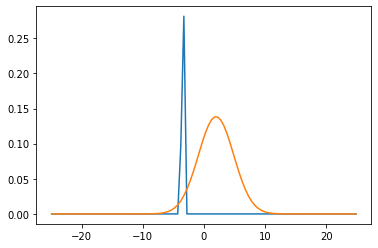
\includegraphics[width=8cm]{two_gauss}
\end{figure}





\end{document}
